\section{Atividade 8}

\subsection{Análise do Diagrama de Bode}

A Figura \ref{fig:Bode} apresenta o diagrama de Bode do sistema massa-mola-amortecedor com os parâmetros \(M = 10\), \(C = 7\), e \(K = 5\). O diagrama de Bode fornece informações valiosas sobre a resposta em frequência do sistema e é composto por dois gráficos: magnitude e fase.

\begin{itemize}
    \item \textbf{Gráfico de Magnitude:}
          O gráfico de magnitude, expresso em decibéis (dB), mostra que a magnitude aumenta inicialmente, atinge um pico em uma determinada frequência e depois decresce. Este comportamento indica a presença de ressonância no sistema, onde a resposta do sistema é maximizada em uma certa frequência.

    \item \textbf{Gráfico de Fase:}
          O gráfico de fase, expresso em graus, apresenta uma variação típica que começa em 0 graus, decresce através de -90 graus e se aproxima de -180 graus em frequências mais altas. A variação da fase indica a diferença de fase entre a entrada e a saída do sistema em diferentes frequências.

    \item \textbf{Margens de Ganho e Fase:}
          \begin{itemize}
              \item \textbf{Margem de Ganho:} A margem de ganho é a quantidade de ganho adicional que o sistema pode tolerar antes de se tornar instável. No gráfico, se a magnitude na frequência onde a fase é -180 graus estiver abaixo de 0 dB, a margem de ganho é positiva e o sistema é estável.
              \item \textbf{Margem de Fase:} A margem de fase é a quantidade de fase adicional que o sistema pode tolerar antes de se tornar instável. No gráfico, se a fase na frequência onde a magnitude é 0 dB estiver acima de -180 graus, a margem de fase é positiva e o sistema é estável.
          \end{itemize}
\end{itemize}

\begin{figure}[h]
    \centering
    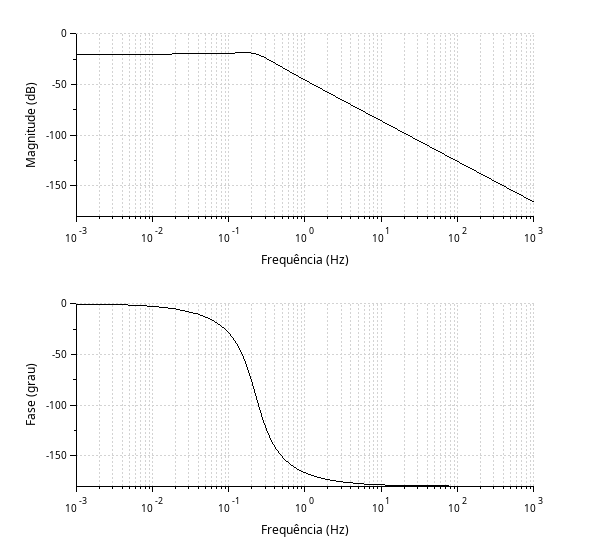
\includegraphics[width=0.8\textwidth]{atividades/8-atividade/assets/bode.png}
    \caption{Diagrama de Bode do sistema massa-mola-amortecedor.}
    \label{fig:Bode}
\end{figure}

A análise do diagrama de Bode sugere que o sistema é estável para as frequências observadas. As margens de ganho e fase indicam que o sistema pode tolerar variações razoáveis no ganho e na fase sem perder a estabilidade. No entanto, é importante considerar que esta análise deve ser complementada com outras técnicas de análise de estabilidade para garantir uma avaliação completa.
